\documentclass[10pt]{beamer}

\usepackage{amsmath}
\usepackage{amssymb}
\usepackage{bm}
\usepackage{hyperref}
\usepackage{csquotes}

\usetheme[progressbar=frametitle]{metropolis}
\usepackage{appendixnumberbeamer}

\usepackage{booktabs}
\usepackage[scale=2]{ccicons}

\usepackage{pgfplots}
\usepgfplotslibrary{dateplot}

\usepackage{xspace}
\newcommand{\themename}{\textbf{\textsc{metropolis}}\xspace}


\DeclareSymbolFont{matha}{OML}{txmi}{m}{it}% txfonts
\DeclareMathSymbol{\varv}{\mathord}{matha}{118}
\usetheme{metropolis}

%\usefonttheme{serif} % default family is serif

\setbeamertemplate{section in toc}[sections numbered]
\setbeamertemplate{subsection in toc}[subsections numbered]

\title{Article presentation :}
\subtitle{Chancel L., Rehm Y., The Carbon Footprint of Capital: Evidence from France, Germany and the US based on Distributional Environmental Accounts}
\author{COMPERAT Étienne  \\ GUGELMO CAVALHEIRO DIAS Paulo \\ ORTIZ Marie Ange}
\institute{Sciences Po}
\date{\today}

\newcommand\ReduceFont{\fontsize{10}{7.2}\selectfont}

\begin{document}

\begin{frame}
    \titlepage
\end{frame}

\begin{frame}
    \ReduceFont
    \frametitle{Outline}
    \tableofcontents[hideallsubsections]
\end{frame}

\section{Introduction}
\begin{frame}
    \tableofcontents[currentsection, hideothersubsections, sections=\value{section}]
\end{frame}

\subsection{Carbon Footprint}
\begin{frame}{\subsecname}
    \begin{columns}
        \begin{column}{0.5\textwidth}
            
\includegraphics[width=1\linewidth, height=0.4\textheight]{../Figures/Camp.png}
            
\includegraphics[width=1\linewidth, height=0.4\textheight]{../Figures/Camp2.png}
        \end{column}
        \begin{column}{0.5\textwidth}
            \textbf{Carbon Footprint:} The measure of the exclusive total amount of emissions of carbon dioxide that is directly and indirectly caused by an activity or is accumulated over the life-cycle stages of a product. \\
            \textbf{Individual Carbon Footprint:} The carbon footprint associated with an individual’s activities, lifestyle or choices. \\
            \textbf{Challenge:} What to include in the carbon footprint? \\
            The Consumption-based Approach
        \end{column}
    \end{columns}
\end{frame}

\subsection{Carbon Footprint of Capital : Chancel and Rehm (2024)}
\begin{frame}{\subsecname}
    \begin{center}
    "The Carbon Footprint of Capital: 
    \textit{Evidence from France, Germany and the US based on Distributional Environmental Accounts}"
    \end{center}

    \textbf{Motivations:}
    \textit{Individuals are not only responsible for their consumption, but also for the assets they own.}
    \begin{enumerate}
        \item Linking carbon emissions to asset ownership to construct a new framework for individual carbon footprint (3 Approaches: Consumption, Ownership and Mixed).
        \item Applying this framework to France, Germany and the US.
        \item Deriving new stylized facts about emissions inequality in the context of environmental and tax policy.
    \end{enumerate}
\end{frame}

\subsection{Key findings}
\begin{frame}{\subsecname}
    \begin{enumerate}
        \item Carbon inequalities are notable in every approach.
        \item In the ownership approach, the majority of emissions for the wealthiest 10\% originates from the assets they own.
        \item Emissions from capital ownership appear to be even more concentrated than capital itself.
    \end{enumerate}
    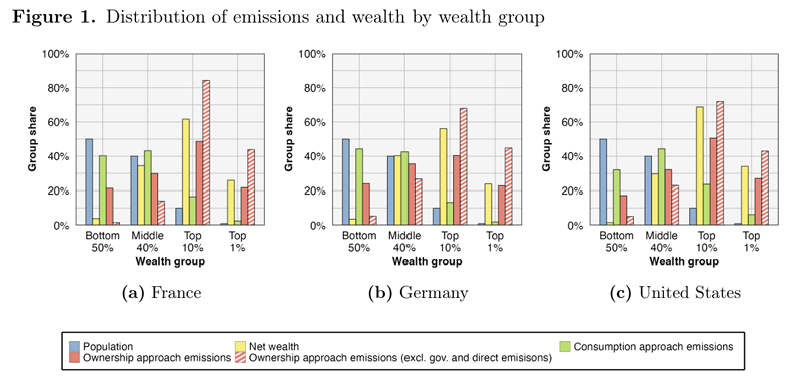
\includegraphics[width=1\linewidth]{../Figures/F1.png}
\end{frame}

\section{Related Literature}
\begin{frame}
    \tableofcontents[currentsection, hideothersubsections, sections=\value{section}]
\end{frame}

\subsection{Measuring the Carbon Footprint}
\begin{frame}{\subsecname}

    \textit{What makes a good Carbon Footprint estimate?}
    
    The 2 fundamentals of carbon accounting:
        \begin{enumerate}
            \item \textbf{Comprehensiveness:} measuring both direct and indirect emissions associated with the economic activity.
            \item \textbf{Exclusivity:} no double-counting.
        \end{enumerate}
    
    Together, these conditions guarantee the \textbf{macro-consistency} of the measures. \\
    So far, the two common ways to measure the carbon footprint have been to focus on \textbf{countries and firms} or \textbf{individuals} (as final consumers).
\end{frame}

\subsection{Consumption-based Approaches}
\begin{frame}{\subsecname}
    \textbf{Individuals' consumption guides the resource allocation in the economy.}
        \begin{itemize}
            \item Underlying assumption: \textit{"Individuals express their preferences through consumption, which sens a signal to producers about what to manufacture and in what quantity."}
            \item The \textbf{"consumer-pays"} principle
        \end{itemize}
        \textbf{Advantage:} Particularly relevant at the country level (accounts for outsourced emissions). \\
        \textbf{Drawback:} Puts the entire responsibility for all emissions on final consumers (despite market failures: lack of information, agency or alternatives).
\end{frame}

\subsection{Production-centered Approaches and Methods of Shared Attribution}
\begin{frame}{\subsecname}
    Contrasting consumption footprints with the production footprints of firms. \\
    \hfill \break
    \textbf{Production-centered approaches}: Focusing on the firm level \\
    Critique: Firms operate through human intervention and individuals are behind their behaviors. $\rightarrow$ \textbf{Ownership-based approach} \\
    \hfill \break
    \textbf{Methods of shared attribution}: Split emissions between consumers and firm owners \\
    Critique: Hard to implement at the individual level. $\rightarrow$ \textbf{Mixed-based approach} \\
    \hfill \break
    \textbf{Income-based carbon accounting}: An alternative at the individual level?
\end{frame}

\subsection{From the Carbon Footprint of individual investment portfolios to the DINA}
\begin{frame}{\subsecname}
    \textit{There already were some attempts at measuring the carbon emissions of individual portfolios (GHG, PCAF). But there exists no consensus regarding these methods and their estimates were not always consistent with aggregate estimates.}
    \vspace{15pt}
    
    Their answer:
    \textbf{the Distributional National and Environmental Accounts (DINA)}
    \begin{itemize}
        \item Goal of the DINA framework: \textit{Reconciling macroeconomic studies (e.g., production, income, wealth) with microeconomic distributional analysis by integrating the study of inequality into the system of national accounts. }
    \end{itemize}
\end{frame}

\section{Data Sources and Methodology}

\begin{frame}{\secname}
    \tableofcontents[currentsection, hideothersubsections, sections=\value{section}]
\end{frame}

% Slide 2: Conceptual Framework
\subsection{Conceptual Framework}
\begin{frame}{\subsecname}
    \textbf{Three Approaches to Carbon Footprints:}
    \begin{itemize}
        \item \textbf{Ownership Approach:} Attributes all direct emissions of firms to their owners.
        \item \textbf{Mixed Approach:} Attributes emissions linked to investment to owners and all others to consumers.
        \item \textbf{Consumption Approach:} Allocates all direct and indirect emissions to consumers.
    \end{itemize}
    \vspace{0.3cm}
    \textbf{Key Principles:}
    \begin{itemize}
        \item \textbf{Consistency:} Aligns with national accounts.
        \item \textbf{Exclusivity:} Ensures no double counting of emissions.
    \end{itemize}
\end{frame}

% Slide 3: Data Sources Overview
\subsection{Data Sources}
\begin{frame}{\subsecname}
    \textbf{Main Data Sources:}
    \begin{itemize}
        \item \textbf{Wealth Data:} HFCS for France and Germany, DINA micro-files for the U.S.
        \item \textbf{Capital Stock:} National accounts data from Eurostat and OECD.
        \item \textbf{Emissions:} Air emission accounts (Eurostat, OECD).
        \item \textbf{Input-Output Tables:} EU-FIGARO dataset for indirect emissions.
        \item \textbf{Cross-Border Investment:} EU-Finflows database and EU-EDGAR.
    \end{itemize}
    \vspace{0.3cm}
    \textbf{Challenges:}
    \begin{itemize}
        \item Surveys underrepresent ultra-wealthy households.
        \item Need for alignment between financial and environmental datasets.
    \end{itemize}
\end{frame}

% Slide 4: Methodology Overview
\subsection{Methodology Overview}
\begin{frame}{\subsecname}
    \textbf{Two Key Steps:}
    \begin{enumerate}
        \item \textbf{Extended Aggregate Environmental Accounts:} Relates emissions to industries, asset classes, and institutional sectors.
        \item \textbf{Distributional Environmental Accounts:} Allocates emissions from institutional sectors to individuals.
    \end{enumerate}
    \vspace{0.3cm}
    \textbf{Key Metrics:}
    \begin{itemize}
        \item Emissions per industry.
        \item Emissions per asset class.
        \item Emissions per wealth group.
    \end{itemize}
\end{frame}

\begin{frame}{\subsecname}
\begin{center}
    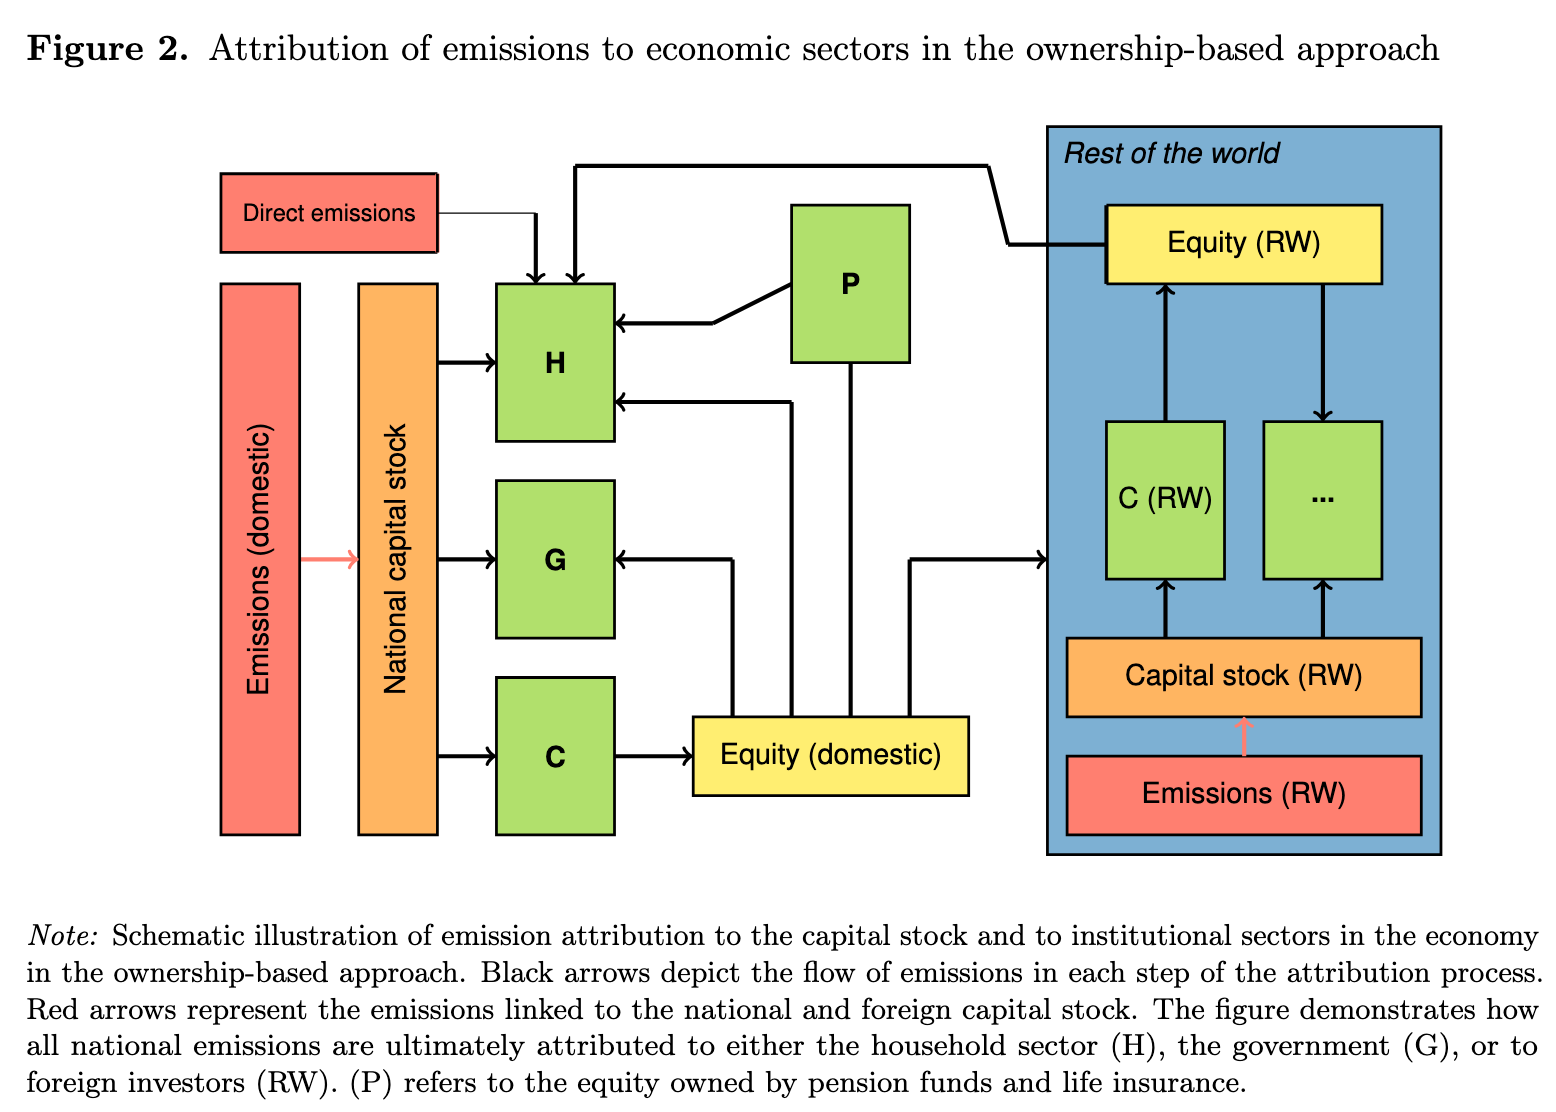
\includegraphics[width=0.9\textwidth]{../Figures/Figure_2.png}
\end{center}
\end{frame}

% Slide 5: Step 1 - Extended Environmental Accounts
\subsubsection{Extended Aggregate Environmental Accounts}
\begin{frame}{\subsubsecname}
    \textbf{Purpose:}
    \begin{itemize}
        \item Calculate total emissions by industry and institutional sector.
        \item Link emissions to the value of the capital stock.
    \end{itemize}
\end{frame}

% Slide 6: Step 2 - Distributional Environmental Accounts
\subsubsection{Distributional Environmental Accounts}
\begin{frame}{\subsubsecname}
    \textbf{Purpose:}
    \begin{itemize}
        \item Distribute total emissions from sectors to individuals.
        \item Attribute emissions based on asset ownership and consumption patterns.
    \end{itemize}

    \textbf{Methodology:}
    \begin{itemize}
        \item \textbf{Ownership Approach:} Allocates emissions directly linked to owned assets.
        \item \textbf{Mixed Approach:} Allocates investment-related emissions to owners, all others to consumers.
        \item \textbf{Consumption Approach:} Allocates all emissions to consumers.
    \end{itemize}
    \vspace{0.3cm}
    \textbf{Challenges:}
    \begin{itemize}
        \item Accurate attribution of emissions for cross-border investments.
        \item Limited data granularity for certain asset classes.
    \end{itemize}
\end{frame}

% Slide 9: Conclusion
\subsection{Conclusion of Section 3}
\begin{frame}{\subsecname}
    \textbf{Key Takeaways:}
    \begin{itemize}
        \item Emission allocation methods depend on robust data and models.
        \item Ownership and mixed approaches provide nuanced insights into emissions inequality.
        \item Data quality and granularity remain critical for future research.
    \end{itemize}
\end{frame}


\section{Carbon Footprint of the Capital}
\begin{frame}{\secname}
    \tableofcontents[currentsection, hideothersubsections, sections=\value{section}]
\end{frame}

\subsection{Capital emissions by industry and institutional sector}

\begin{frame}{\subsecname}
    \begin{columns}
        \begin{column}{0.5\textwidth}
            Industries :
                \begin{itemize}
                    \item Agriculture and mining
                    \item Energy, water and waste
                    \item Manufacturing
                    \item Transport
                    \item Real estate and construction
                    \item Health and education
                    \item Public administration
                    \item Services
                \end{itemize}
        \end{column}
        \begin{column}{0.5\textwidth}
            \ReduceFont
            Results : 
                \begin{itemize}
                    \item Manufacturing as the largest emitting sector in FR and DE
                    \item Agriculture and mining as the largest emitting sector in the US
                    \item Agriculture and mining as the most carbon-intensive sector
                    \item Similar carbon intensity for the manufacturing sector
                    \item Difference in definition for the Real Estate and Construction sector
                \end{itemize}    
        \end{column}
    \end{columns}
    \hfill \break
    Following : Table 1, Emission intensities by industry groups
\end{frame}

\begin{frame}{\subsecname}
    \begin{center}
        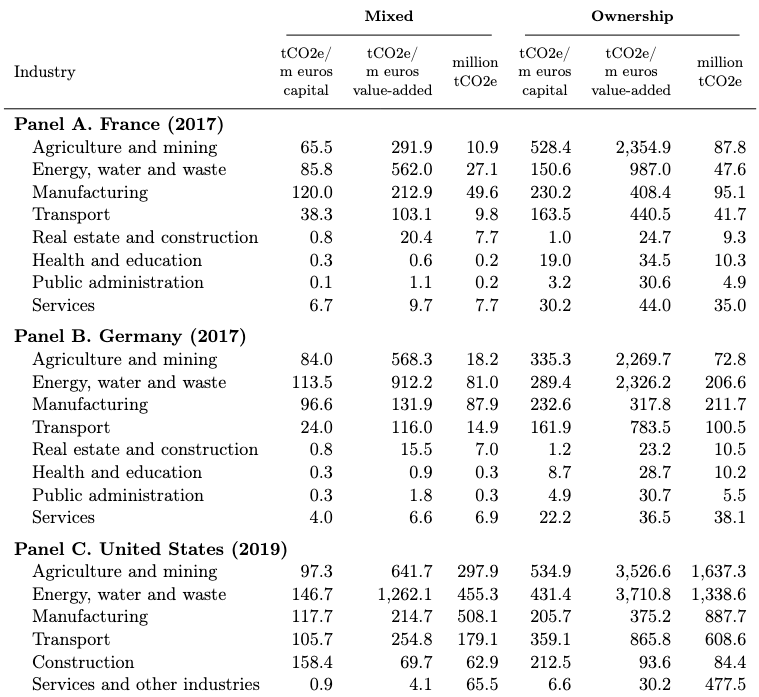
\includegraphics[height=0.9\textheight]{../Figures/T1.png}    
    \end{center}
\end{frame}

\subsection{Capital emissions by asset class}

\begin{frame}{\subsecname}
    \begin{columns}
        \begin{column}{0.5\textwidth}
            Assets :
                \begin{itemize} 
                    \item Housing assets
                    \item Business assets
                    \item Equities 
                    \item Pension assets
                    \item Fixed income assets
                \end{itemize}
        \end{column}
        \begin{column}{0.5\textwidth}
            \ReduceFont
            Results : 
                \begin{itemize}
                    \item Equity is the most polluting asset class.
                    \item Pension assets are the second most polluting asset class.
                    \item Business assets are the third most polluting asset class.
                    \item Housing has an important market valuation, but emits little.
                    \item Important intensity of pension assets for Germany.
                \end{itemize}    
        \end{column}
    \end{columns}
    \hfill \break
    In clear, there exist important differences between types of assets.
\end{frame}

\begin{frame}{\subsecname}
    \begin{center}
        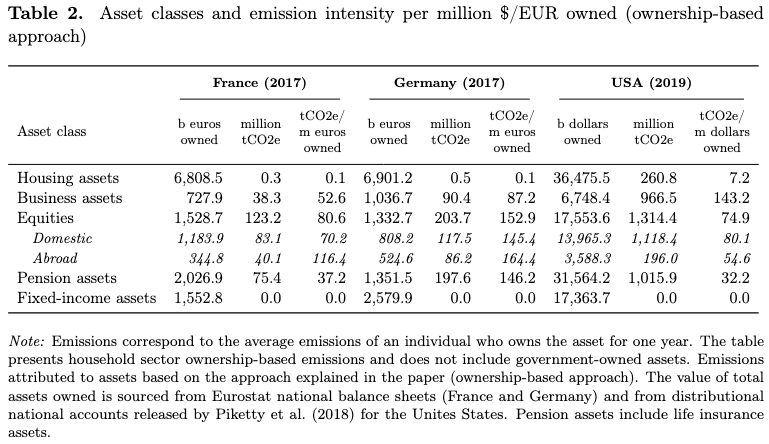
\includegraphics[width=\textwidth]{../Figures/T2.png}    
    \end{center}
\end{frame}

\subsection{The role of foreign capital in national emissions}
\begin{frame}{\subsecname}
    \begin{itemize}
        \item In France and in the US, equity held abroad represents about 20-25\% of owned equities.
        \item In Germany, equity held abroad represents about 40\% of owned equities.
        \item Foreign equity held by French and German citizens are more carbon intensive than those owned by the US citizens.
    \end{itemize}
\end{frame}

\section{The Distribution of Carbon Footprints}
\begin{frame}{\secname}
    \tableofcontents[currentsection, hideothersubsections, sections=\value{section}]
\end{frame}

\subsection{Emissions rise with income and wealth}
\begin{frame}{\subsecname}
    \begin{columns}
        \begin{column}{0.5\textwidth}
            Generally :
            \begin{itemize}
                \item Emissions are positively correlated with wealth.
                \item Consumption approach : carbon inequalities are less concentrated than income.
                \item Mixed-based approach : carbon inequalities are as concentrated as income.
                \item Ownership approach : carbon inequalities are more concentrated than wealth.
            \end{itemize}
        \end{column}
        \begin{column}{0.5\textwidth}
            \ReduceFont
            International comparison :
            \begin{itemize}
                \item The US are more carbon inequal than Germany, which is more carbon inequal than France.
                \item The majority of the US emit as much as the top of the distribution of France and Germany in the two first approaches.
                \item The top French group emits less despite owning more of the national equity than their German counterpart.
            \end{itemize}
        \end{column}
    \end{columns}
\end{frame}

\begin{frame}{\subsecname}
    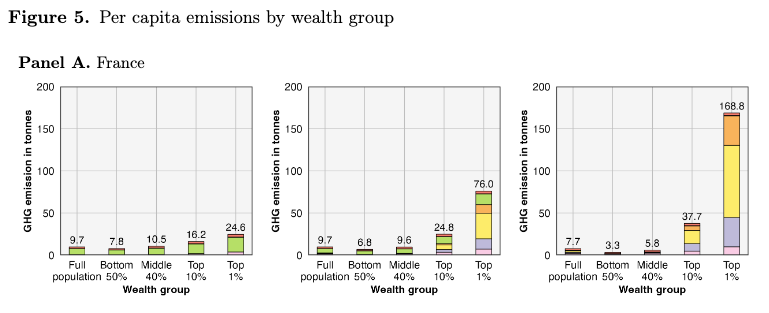
\includegraphics[width=\textwidth]{../Figures/F51.png}
\end{frame}

\begin{frame}{\subsecname}
    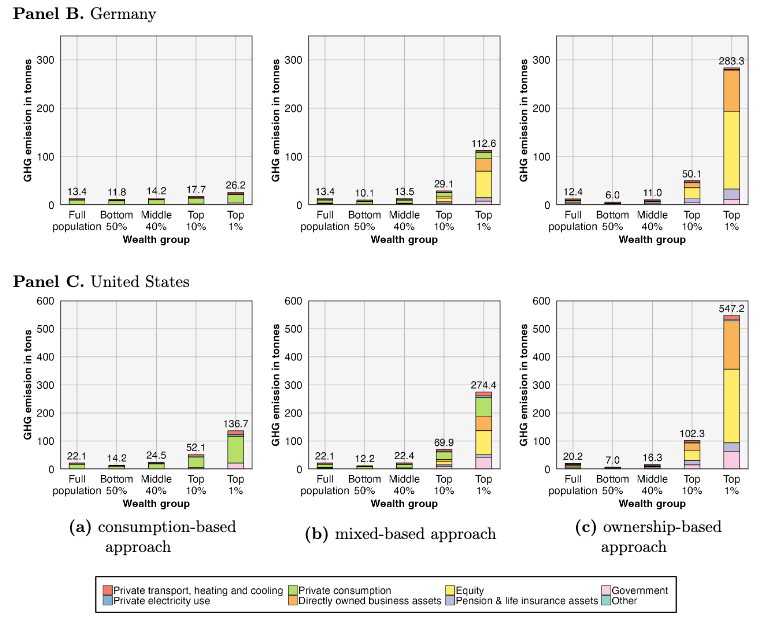
\includegraphics[width=\textwidth, height=0.9\textheight]{../Figures/F52.png}
\end{frame}

\subsection{Emissions intensity rises with wealth}
\begin{frame}{\subsecname}
    Average emission intensity tends to increase alongside with wealth at the very top of the distribution.
    This explains the greater concentration of carbon emissions compared to wealth.
    \begin{center}
        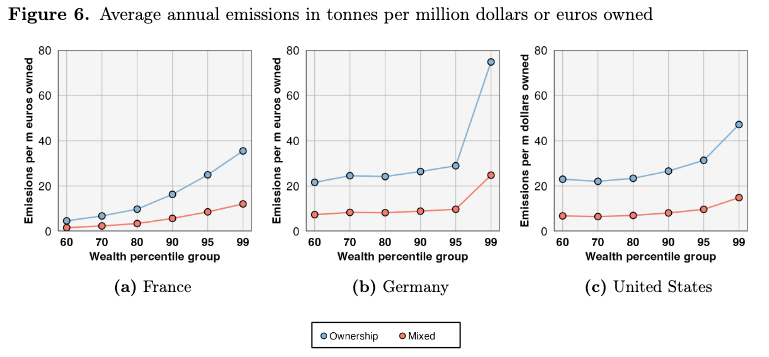
\includegraphics[width=0.9\textwidth]{../Figures/F6.png}
    \end{center}
\end{frame}

\subsection{The weight of capital emissions among top groups}

\begin{frame}{\subsecname}
    \begin{itemize}
        \item Importance of the emissions of top groups.
        \item Emissions of the top 1\% (p.36) :
        \begin{table}[!ht]
            \centering
            \begin{tabular}{|l|l|l|l|l|}
            \hline
                Countries & Consumption & Ownership & Multiplication in tCO2e \\ \hline
                France & 2.5\% & 21.5\% & 6 \\ \hline
                Germany & 2\% & 22.3\% & 11 \\ \hline
                US & 6.2\% & 26.9\% & 16 \\ \hline
            \end{tabular}
        \end{table}
        \item Key role of Capital ownership in the determinant of the top of the distribution.
        \item Structure of the emissions alongside the wealth distribution.
    \end{itemize}
\end{frame}

\begin{frame}{\subsecname}
    \begin{center}
        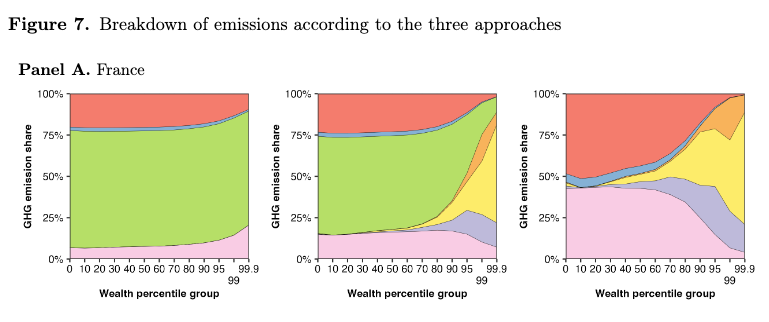
\includegraphics[width=0.9\textwidth]{../Figures/F71.png}
    \end{center}
\end{frame}

\begin{frame}{\subsecname}
    \begin{center}
        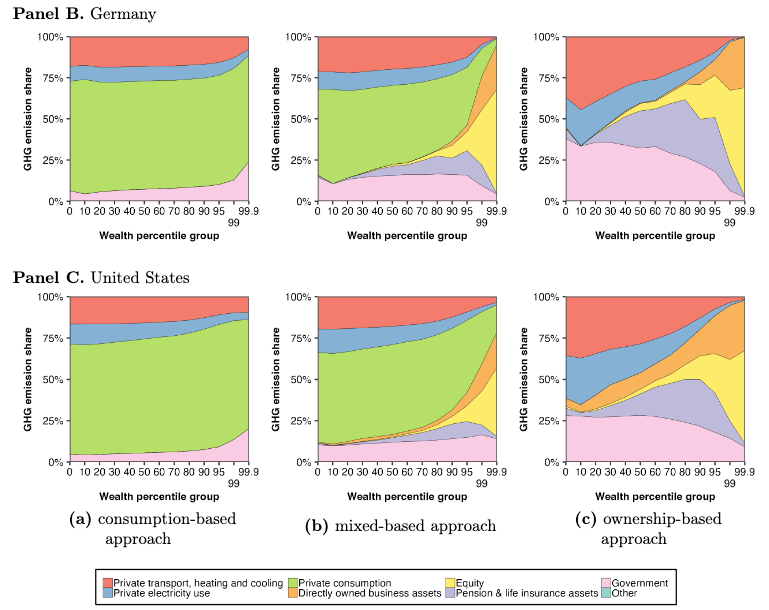
\includegraphics[width=0.9\textwidth]{../Figures/F72.png}
    \end{center}
\end{frame}

\section{Discussion}

\begin{frame}{\secname}
    \tableofcontents[currentsection, hideothersubsections, sections=\value{section}]
\end{frame}

\subsection{Robustness of the results}
\begin{frame}{\subsecname}
    \textbf{Robustness checks}
    \textit{Even under extreme combinations of assumptions, the general patterns observed hold, in particular that accounting for ownership-based emission footprints increases emission inequality considerably.}
    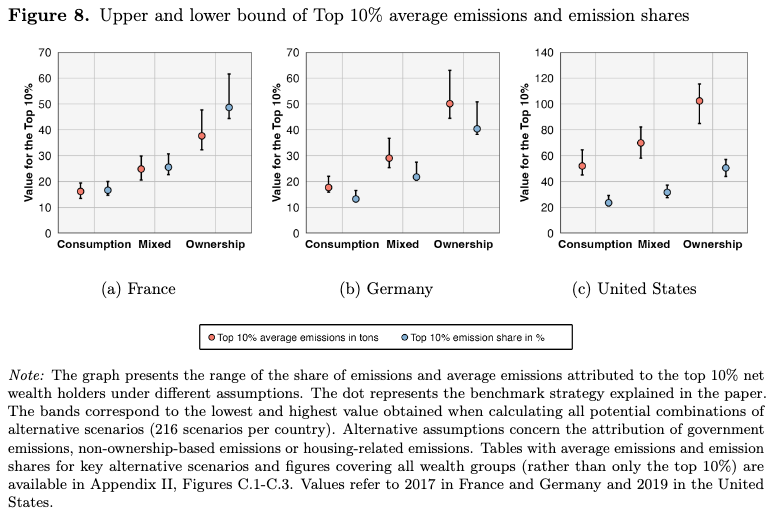
\includegraphics[width=1\linewidth]{../Figures/Figure_8.png}
\end{frame}

\subsection{Scopes and limitations}

\subsubsection{Limitations due to the data}

% Slide 3: Incomplete Data for High-Wealth Individuals
\begin{frame}{\subsecname \  - \subsubsecname}
    Incomplete Data for High-Wealth Individuals \\ 
    \textbf{Issue :}
    \begin{itemize}
        \item Surveys like HFCS and DINA underrepresent the top 1\% of wealth holders.
        \item This underestimates emissions linked to equity and business assets.
    \end{itemize}
    \vspace{0.3cm}
    \textbf{Discussion :}
    \begin{itemize}
        \item Integrate alternative data sources (e.g., tax records, billionaire lists).
        \item Refine attribution of emissions to high-net-worth individuals.
    \end{itemize}
    \vspace{0.3cm}
    \textbf{Impact:}
    \begin{itemize}
        \item Potential bias in emissions share attributed to the wealthiest.
    \end{itemize}
\end{frame}

% Slide 4: Sensitivity to Assumptions
\begin{frame}{\subsecname \  - \subsubsecname}
    Sensitivity to Assumptions \\ 
    \textbf{Issue :}
    \begin{itemize}
        \item Allocation of government emissions varies (proportional to income vs. lump-sum distribution).
        \item Cross-border investments use average intensities, ignoring sector-specific differences.
    \end{itemize}
    \vspace{0.3cm}
    \textbf{Discussion :}
    \begin{itemize}
        \item Tested alternative assumptions for government emissions:
        \begin{itemize}
            \item Proportional to income: increases share of emissions for wealthy groups.
            \item Lump sum: reduces their share.
        \end{itemize}
        \item Importance of robust sensitivity analysis.
    \end{itemize}
\end{frame}

% Slide 5: Lack of Granularity in Asset Data
\begin{frame}{\subsecname \  - \subsubsecname}
    Lack of Granularity in Asset Data \\ 
    \textbf{Issue :}
    \begin{itemize}
        \item No differentiation between carbon-intensive and low-carbon investments.
        \item Masks the role of sustainable finance in reducing emissions.
    \end{itemize}
    \vspace{0.3cm}
    \textbf{Discussion :}
    \begin{itemize}
        \item Propose linking firm-level environmental data to financial datasets.
        \item Enables better identification of green vs. carbon-intensive portfolios.
    \end{itemize}
    \vspace{0.3cm}
    \textbf{Impact:}
    \begin{itemize}
        \item Improved insights into the role of individual investment behavior.
    \end{itemize}
\end{frame}

% Slide 6: Challenges with Cross-Border Investments
\begin{frame}{\subsecname \  - \subsubsecname}
    Challenges with Cross-Border Investments \\
    \textbf{Issue :}
    \begin{itemize}
        \item Relies on average carbon intensities by country.
        \item Ignores sector-specific variations in foreign economies.
    \end{itemize}
    \vspace{0.3cm}
    \textbf{Discussion :}
    \begin{itemize}
        \item Highlighted uncertainty in emissions from foreign equity.
        \item Proposed improvements:
        \begin{itemize}
            \item Granular international investment data.
            \item Sector-specific emissions intensities for cross-border assets.
        \end{itemize}
    \end{itemize}
\end{frame}

% Slide 7: Dependence on Static Models
\begin{frame}{\subsecname \  - \subsubsecname}
    Dependence on Static Models \\
    \textbf{Issue :}
    \begin{itemize}
        \item Relies on static multi-regional input-output models (MRIOs).
        \item Assumes linear relationships between inputs and emissions.
    \end{itemize}
    \vspace{0.3cm}
    \textbf{Discussion :}
    \begin{itemize}
        \item Recommends dynamic or hybrid models.
        \item These models require richer datasets, currently unavailable.
    \end{itemize}
    \vspace{0.3cm}
    \textbf{Impact:}
    \begin{itemize}
        \item Limits ability to capture feedback effects and technological change.
    \end{itemize}
\end{frame}

\subsubsection{Interpretative Limitations and Individual Responsibility}
\begin{frame}{\subsecname \  - \subsubsecname}

    \textbf{Carbon footprint and individual responsibility:} \\ 
    No broadly defined individual footprinting approach can fully capture the actual responsibility individual bears for emissions. \\

    The three conditions for individual responsibility:
    \begin{itemize}
        \item Agency
        \item Intentionality
        \item Alternatives
    \end{itemize}

    In reality, these conditions are rarely met. \\

    A potential way to account for individual responsibility:
    \begin{itemize}
        \item $\alpha$: rate of control over indirect emissions embedded in individual consumption
        \item $\beta$: rate of agency and control over direct emissions embedded in direct consumption 
    \end{itemize}

    \vspace{5pt}
    The role of the government in decarbonization.
\end{frame}

\subsection{Stylized facts on inequality and emissions}
\begin{frame}{\subsecname}

    \begin{enumerate}
        \item \textbf{Challenging the Kuznets curve}: a pronounced economic gradient linked to emissions.

            \textit{Emissions do not decline after a certain income level.}
            \vspace{5pt}

        \item \textbf{Consumption-based emissions are less concentrated than income and wealth.}
        
            \textit{Because wealthier individuals consume a smaller fraction (and wealth) than less well-off individuals.}
            \vspace{5pt}

        \item \textbf{Wealth emissions are even more concentrated than wealth itself.}
        
            \textit{Because the type of assets owned by the bottom 90$\%$ (mostly housing and deposits) have low or zero carbon intensity.}
            \vspace{5pt}

    \end{enumerate}

\end{frame}


\subsection{Distributional properties and revenue estimates for a carbon wealth tax}
\begin{frame}{\subsecname}
    So far, climate tax policy mirrors the approaches taken in the climate inequality literature, which have not considered the role of the individual.
    \textbf{A 150 euro/dollars "per tonne" tax on the carbon content of assets}
    \begin{center}
        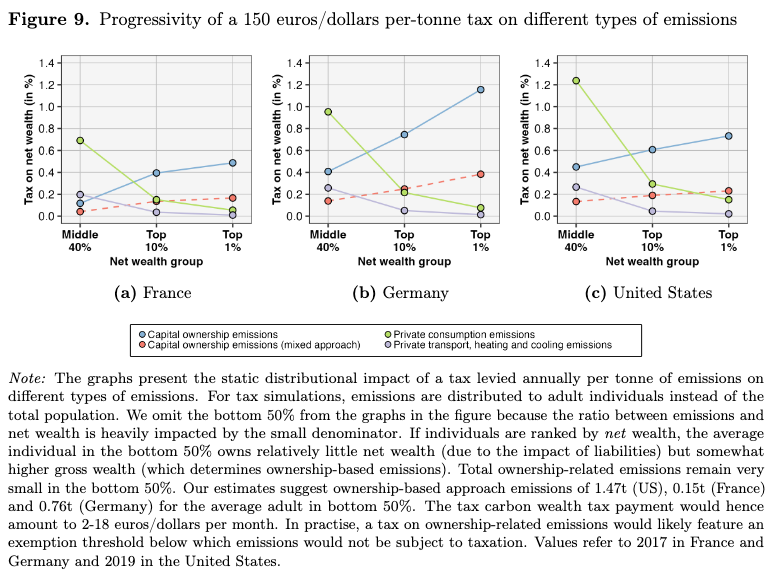
\includegraphics[width=1\textwidth]{../Figures/Figure_9.png}
    \end{center}
\end{frame}


\section{Conclusion}
\begin{frame}{\secname}
    \begin{itemize}
        \item Complementarity of the three approaches, way to analyse emissions inequality.
        \item Calling for a broader theory on optimal taxation based on capital carbon emissions. 
    \end{itemize}
\end{frame}

\end{document}